\documentclass[aspectratio=169]{beamer}

\usetheme{default}
\usecolortheme{dove}

\setbeamertemplate{navigation symbols}{}
\setbeamertemplate{footline}{%
  \hfill{\large\insertframenumber\,/\,\inserttotalframenumber}\hspace{0.8em}\vspace{0.5em}%
}

\definecolor{popblue}{RGB}{52, 101, 164}
\definecolor{sampred}{RGB}{204, 0, 0}
\definecolor{paramgreen}{RGB}{0, 140, 70}
\definecolor{warnred}{RGB}{180, 40, 40}
\definecolor{orange1}{RGB}{220, 120, 0}
\definecolor{violet1}{RGB}{120, 50, 160}
\definecolor{lightbg}{RGB}{245, 245, 250}

\setbeamercolor{frametitle}{fg=popblue}
\setbeamercolor{title}{fg=popblue}

\usepackage{pgfplots}
\usepackage{tikz}
\usetikzlibrary{shapes, arrows.meta, positioning, calc, decorations.pathreplacing, patterns}
\pgfplotsset{compat=1.18}
\usepackage{amsmath, amssymb}
\usepackage{fontenc}

\title{Lecture 8: The Bootstrap}
\subtitle{Resampling $\cdot$ Bootstrap CIs $\cdot$ Permutation Tests}
\date{}

\begin{document}

% ============================================================
\begin{frame}
\titlepage
\end{frame}

% ============================================================
\begin{frame}
\frametitle{Previously, on Lecture 7\ldots}

\begin{center}
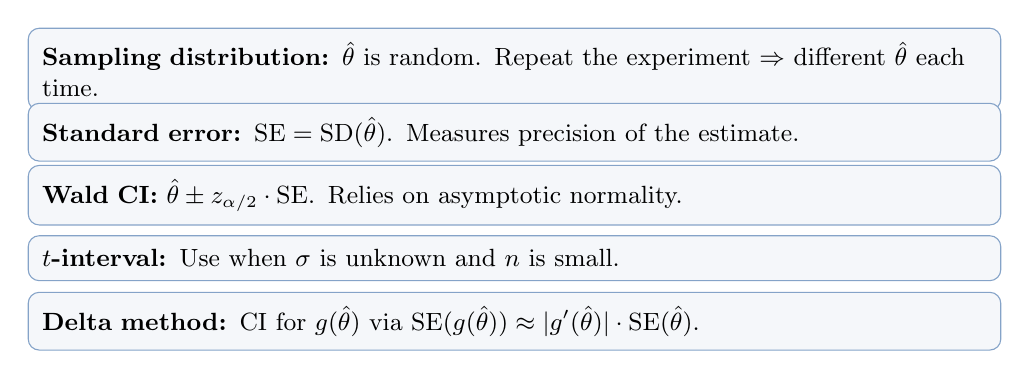
\begin{tikzpicture}[
  sbox/.style={draw=popblue!60, fill=popblue!5, rounded corners=4pt, text width=12cm, minimum height=0.5cm, align=left, inner sep=5pt, font=\small}
]
  \node[sbox] at (0, 2.0) {\textbf{Sampling distribution:} $\hat\theta$ is random. Repeat the experiment $\Rightarrow$ different $\hat\theta$ each time.};
  \node[sbox] at (0, 1.2) {\textbf{Standard error:} $\text{SE} = \text{SD}(\hat\theta)$. Measures precision of the estimate.};
  \node[sbox] at (0, 0.4) {\textbf{Wald CI:} $\hat\theta \pm z_{\alpha/2}\cdot\text{SE}$. Relies on asymptotic normality.};
  \node[sbox] at (0, -0.4) {\textbf{$t$-interval:} Use when $\sigma$ is unknown and $n$ is small.};
  \node[sbox] at (0, -1.2) {\textbf{Delta method:} CI for $g(\hat\theta)$ via $\text{SE}(g(\hat\theta)) \approx |g'(\hat\theta)|\cdot\text{SE}(\hat\theta)$.};
\end{tikzpicture}
\end{center}

\vspace{0.3cm}
\begin{center}
{\large\textbf{Today:}} What if there's \textbf{no formula} for the SE?\\[4pt]
What if the sampling distribution isn't Normal? What if the statistic is complicated?
\end{center}
\end{frame}

% ============================================================
\begin{frame}
\frametitle{The Problem}
\begin{center}
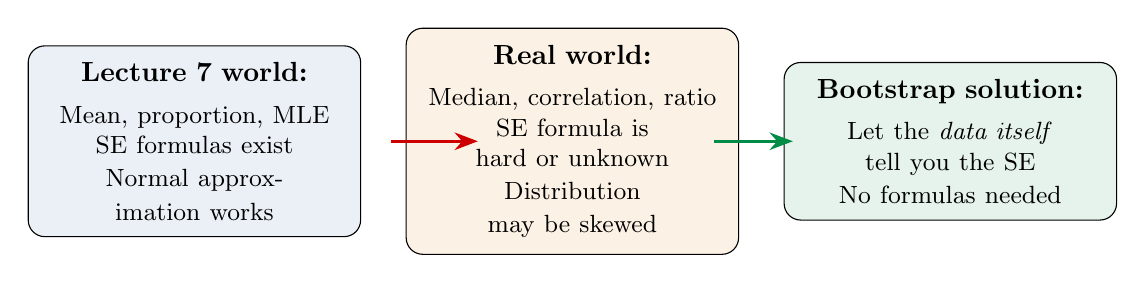
\begin{tikzpicture}[
  box/.style={draw, rounded corners=6pt, minimum width=4cm, minimum height=2cm, align=center, text width=3.8cm, inner sep=6pt}
]
  \node[box, fill=popblue!10] at (-4.8, 0) {
    \textbf{Lecture 7 world:}\\[4pt]
    \small Mean, proportion, MLE\\
    SE formulas exist\\
    Normal approximation works
  };

  \node[box, fill=orange1!10] at (0, 0) {
    \textbf{Real world:}\\[4pt]
    \small Median, correlation, ratio\\
    SE formula is hard or unknown\\
    Distribution may be skewed
  };

  \node[box, fill=paramgreen!10] at (4.8, 0) {
    \textbf{Bootstrap solution:}\\[4pt]
    \small Let the \textit{data itself}\\
    tell you the SE\\
    No formulas needed
  };

  \draw[-{Stealth}, very thick, sampred] (-2.3, 0) -- (-1.2, 0);
  \draw[-{Stealth}, very thick, paramgreen] (1.8, 0) -- (2.8, 0);
\end{tikzpicture}
\end{center}
\end{frame}

% ============================================================
\section{The Bootstrap Idea}

\begin{frame}
\begin{center}
  \vspace{2cm}
  {\Huge\bfseries\textcolor{popblue}{The Bootstrap Idea}}

  \vspace{0.8cm}
  {\large ``Pull yourself up by your own bootstraps''}
\end{center}
\end{frame}

\begin{frame}
\frametitle{The Core Insight}

\begin{center}
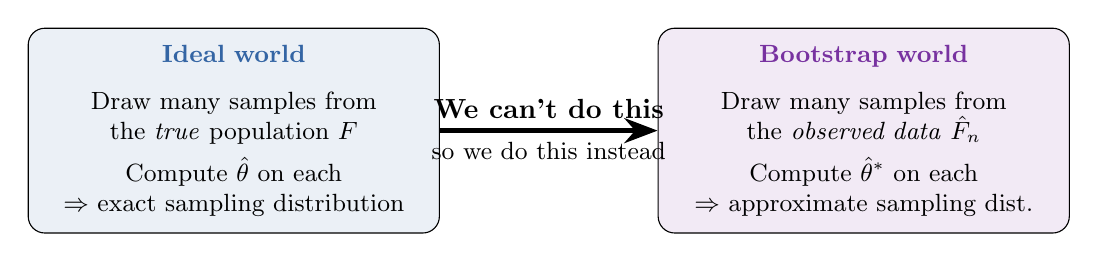
\begin{tikzpicture}[
  rbox/.style={draw, rounded corners=6pt, minimum width=5cm, minimum height=2cm, align=center, text width=4.8cm, inner sep=6pt, font=\small}
]
  \node[rbox, fill=popblue!10] (ideal) at (-4, 0) {
    \textbf{\textcolor{popblue}{Ideal world}}\\[6pt]
    Draw many samples from\\
    the \textit{true} population $F$\\[4pt]
    Compute $\hat\theta$ on each\\
    $\Rightarrow$ exact sampling distribution
  };

  \node[rbox, fill=violet1!10] (boot) at (4, 0) {
    \textbf{\textcolor{violet1}{Bootstrap world}}\\[6pt]
    Draw many samples from\\
    the \textit{observed data} $\hat{F}_n$\\[4pt]
    Compute $\hat\theta^*$ on each\\
    $\Rightarrow$ approximate sampling dist.
  };

  \draw[-{Stealth}, very thick, line width=2pt] (ideal) -- (boot)
    node[midway, above, font=\normalsize\bfseries] {We can't do this}
    node[midway, below, font=\small] {so we do this instead};
\end{tikzpicture}
\end{center}

\vspace{0.3cm}
\pause
\begin{center}
\fcolorbox{orange1}{orange1!5}{\parbox{10cm}{\centering\small
  \textbf{Key idea:} The empirical distribution $\hat{F}_n$ is our best estimate of $F$.\\[2pt]
  Sampling from $\hat{F}_n$ $=$ sampling \textbf{with replacement} from the data.
}}
\end{center}
\end{frame}

\begin{frame}
\frametitle{The Bootstrap Algorithm}

\begin{center}
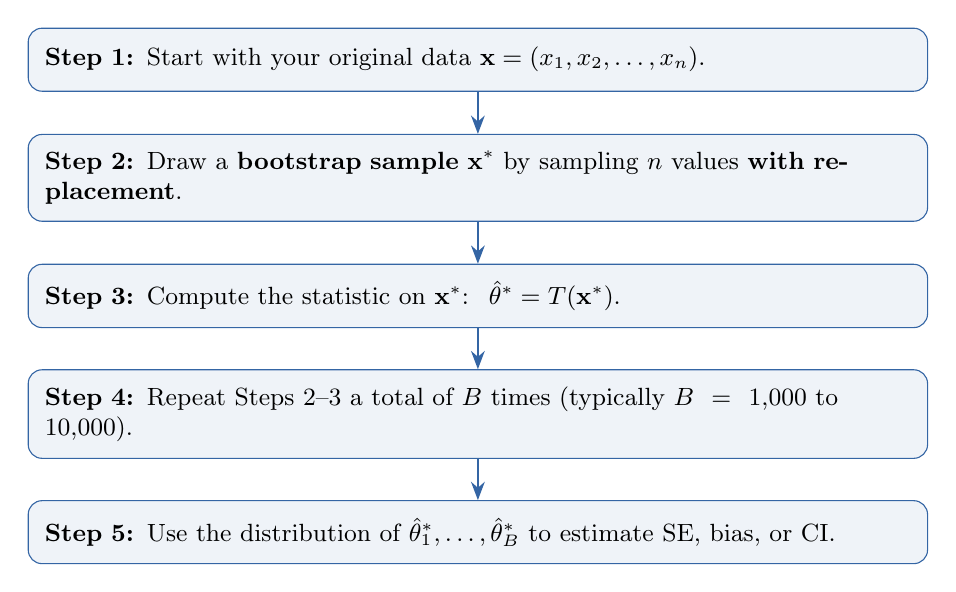
\begin{tikzpicture}[
  stp/.style={draw=popblue, fill=popblue!8, rounded corners=5pt, text width=11cm, minimum height=0.8cm, align=left, inner sep=6pt, font=\small}
]
  \node[stp] (s1) at (0, 3) {\textbf{Step 1:} Start with your original data $\mathbf{x} = (x_1, x_2, \ldots, x_n)$.};
  \pause
  \node[stp] (s2) at (0, 1.5) {\textbf{Step 2:} Draw a \textbf{bootstrap sample} $\mathbf{x}^*$ by sampling $n$ values \textbf{with replacement}.};
  \pause
  \node[stp] (s3) at (0, 0) {\textbf{Step 3:} Compute the statistic on $\mathbf{x}^*$: $\;\hat\theta^* = T(\mathbf{x}^*)$.};
  \pause
  \node[stp] (s4) at (0, -1.5) {\textbf{Step 4:} Repeat Steps 2--3 a total of $B$ times (typically $B = 1{,}000$ to $10{,}000$).};
  \pause
  \node[stp] (s5) at (0, -3) {\textbf{Step 5:} Use the distribution of $\hat\theta_1^*, \ldots, \hat\theta_B^*$ to estimate SE, bias, or CI.};

  \draw[-{Stealth}, thick, popblue] (s1) -- (s2);
  \draw[-{Stealth}, thick, popblue] (s2) -- (s3);
  \draw[-{Stealth}, thick, popblue] (s3) -- (s4);
  \draw[-{Stealth}, thick, popblue] (s4) -- (s5);
\end{tikzpicture}
\end{center}
\end{frame}

\begin{frame}
\frametitle{Visualizing a Bootstrap Sample}

\small
\textbf{Original data:} $\mathbf{x} = (2, 5, 7, 3, 8, 1, 6)$, \; $n = 7$.

\vspace{0.3cm}
\begin{center}
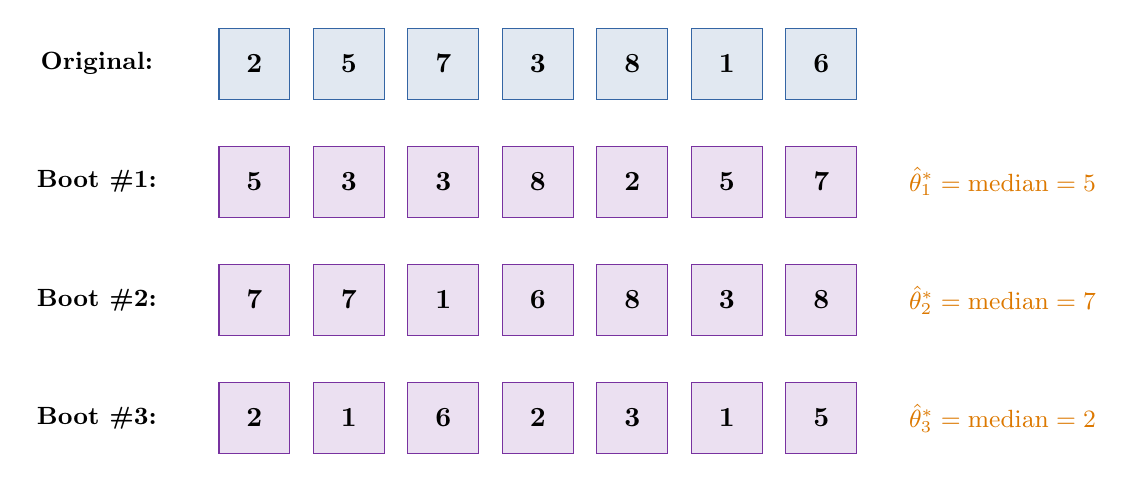
\begin{tikzpicture}[
  dbox/.style={draw=popblue, fill=popblue!15, minimum width=0.9cm, minimum height=0.9cm, font=\normalsize\bfseries},
  bbox/.style={draw=violet1, fill=violet1!15, minimum width=0.9cm, minimum height=0.9cm, font=\normalsize\bfseries}
]
  % Original
  \node[font=\small\bfseries] at (-2, 0) {Original:};
  \foreach \val [count=\i from 0] in {2, 5, 7, 3, 8, 1, 6} {
    \node[dbox] at (\i*1.2, 0) {\val};
  }

  \pause
  % Bootstrap sample 1
  \node[font=\small\bfseries] at (-2, -1.5) {Boot \#1:};
  \foreach \val [count=\i from 0] in {5, 3, 3, 8, 2, 5, 7} {
    \node[bbox] at (\i*1.2, -1.5) {\val};
  }
  \node[font=\small, orange1] at (9.5, -1.5) {$\hat\theta^*_1 = \text{median} = 5$};

  \pause
  % Bootstrap sample 2
  \node[font=\small\bfseries] at (-2, -3) {Boot \#2:};
  \foreach \val [count=\i from 0] in {7, 7, 1, 6, 8, 3, 8} {
    \node[bbox] at (\i*1.2, -3) {\val};
  }
  \node[font=\small, orange1] at (9.5, -3) {$\hat\theta^*_2 = \text{median} = 7$};

  \pause
  % Bootstrap sample 3
  \node[font=\small\bfseries] at (-2, -4.5) {Boot \#3:};
  \foreach \val [count=\i from 0] in {2, 1, 6, 2, 3, 1, 5} {
    \node[bbox] at (\i*1.2, -4.5) {\val};
  }
  \node[font=\small, orange1] at (9.5, -4.5) {$\hat\theta^*_3 = \text{median} = 2$};
\end{tikzpicture}
\end{center}

\vspace{0.2cm}
\small Note: some values appear \textbf{multiple times}, others \textbf{not at all}. That's ``with replacement.''
\end{frame}

\begin{frame}
\frametitle{Bootstrap Distribution of the Median}

\begin{center}
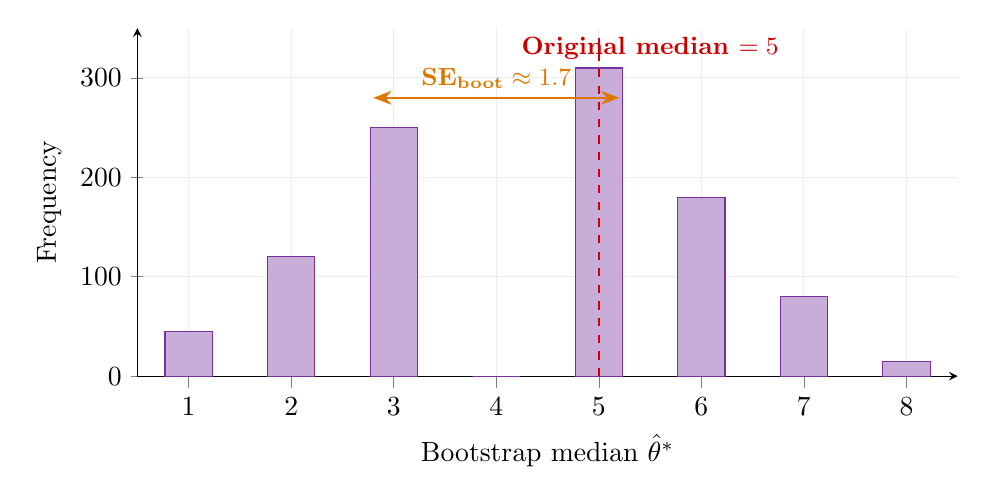
\begin{tikzpicture}
  \begin{axis}[
    width=12cm, height=6cm,
    xlabel={Bootstrap median $\hat\theta^*$},
    ylabel={Frequency},
    ymin=0, ymax=350,
    xmin=0.5, xmax=8.5,
    axis lines=left,
    grid=major, grid style={gray!15},
    xtick={1,2,3,4,5,6,7,8},
    ytick={0, 100, 200, 300},
    bar width=0.6cm,
    ybar,
  ]
    % Simulated bootstrap distribution of median for (2,5,7,3,8,1,6)
    \addplot[fill=violet1!40, draw=violet1] coordinates {
      (1, 45) (2, 120) (3, 250) (4, 0) (5, 310) (6, 180) (7, 80) (8, 15)
    };

    % Original median
    \draw[thick, sampred, dashed] (axis cs:5, 0) -- (axis cs:5, 340);
    \node[font=\small\bfseries, sampred] at (axis cs:5.5, 330) {Original median $= 5$};

    % SE annotation
    \draw[{Stealth}-{Stealth}, thick, orange1] (axis cs:2.8, 280) -- (axis cs:5.2, 280);
    \node[font=\small\bfseries, orange1, above] at (axis cs:4, 280) {$\text{SE}_{\text{boot}} \approx 1.7$};
  \end{axis}
\end{tikzpicture}
\end{center}

\small The \textbf{spread} of the bootstrap distribution estimates the standard error.\\
No formula needed --- just simulation!
\end{frame}

% ============================================================
\section{Bootstrap Standard Errors and Bias}

\begin{frame}
\begin{center}
  \vspace{2cm}
  {\Huge\bfseries\textcolor{popblue}{Bootstrap SE \& Bias}}

  \vspace{0.8cm}
  {\large Estimating uncertainty from the data}
\end{center}
\end{frame}

\begin{frame}
\frametitle{Bootstrap Standard Error}

\begin{center}
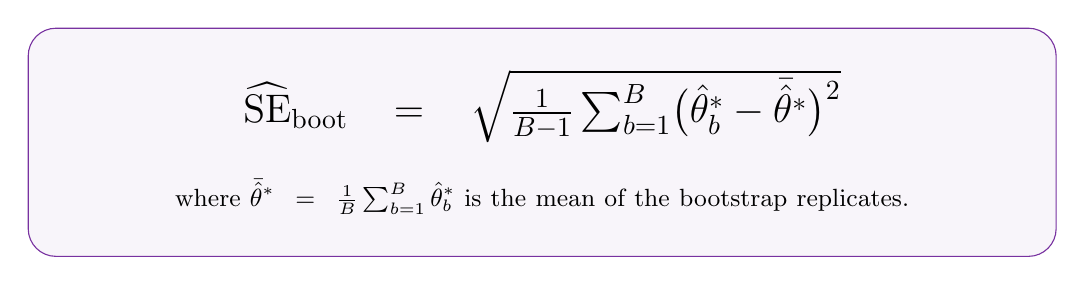
\begin{tikzpicture}
  \node[draw=violet1, fill=violet1!5, rounded corners=10pt, text width=12cm, align=center, inner sep=15pt] {
    {\Large
    $\widehat{\text{SE}}_{\text{boot}} = \sqrt{\frac{1}{B-1}\sum_{b=1}^{B}\bigl(\hat\theta_b^* - \bar{\hat\theta}^*\bigr)^2}$
    }\\[12pt]
    \small where $\bar{\hat\theta}^* = \frac{1}{B}\sum_{b=1}^B \hat\theta_b^*$ is the mean of the bootstrap replicates.
  };
\end{tikzpicture}
\end{center}

\vspace{0.5cm}
\pause
\begin{center}
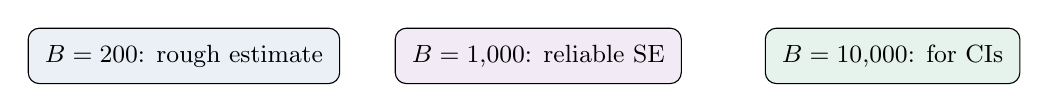
\begin{tikzpicture}[
  cbox/.style={draw, rounded corners=4pt, align=center, font=\small, inner sep=6pt}
]
  \node[cbox, fill=popblue!10] at (-4.5, 0) {$B = 200$: rough estimate};
  \node[cbox, fill=violet1!10] at (0, 0) {$B = 1{,}000$: reliable SE};
  \node[cbox, fill=paramgreen!10] at (4.5, 0) {$B = 10{,}000$: for CIs};
\end{tikzpicture}
\end{center}

\vspace{0.2cm}
\centering\small
More $B$ = more precision in the SE estimate. The cost is purely computational.
\end{frame}

\begin{frame}
\frametitle{Bootstrap Bias Estimation}

\small
The bootstrap can also estimate \textbf{bias}:

\vspace{0.2cm}
\begin{center}
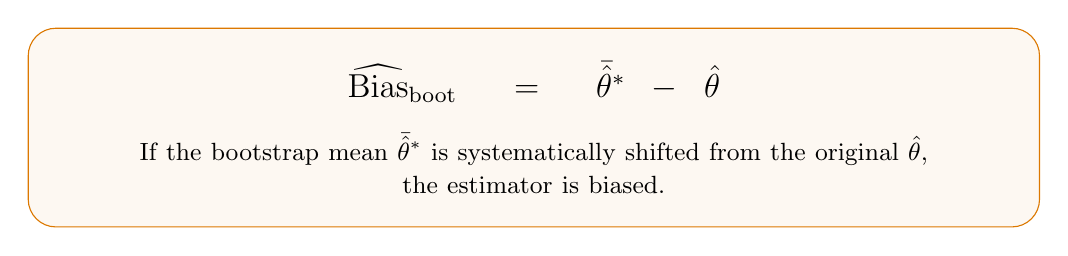
\begin{tikzpicture}
  \node[draw=orange1, fill=orange1!5, rounded corners=10pt, text width=12cm, align=center, inner sep=12pt] {
    {\large
    $\widehat{\text{Bias}}_{\text{boot}} = \bar{\hat\theta}^* - \hat\theta$
    }\\[10pt]
    \small If the bootstrap mean $\bar{\hat\theta}^*$ is systematically shifted from the original $\hat\theta$,\\
    the estimator is biased.
  };
\end{tikzpicture}
\end{center}

\vspace{0.3cm}
\pause
\textbf{Bias-corrected estimate:}
$$\hat\theta_{\text{corrected}} = \hat\theta - \widehat{\text{Bias}}_{\text{boot}} = 2\hat\theta - \bar{\hat\theta}^*$$

\vspace{0.1cm}
\pause
\begin{center}
\fcolorbox{warnred}{warnred!5}{\parbox{10cm}{\centering\small
  \textbf{Caution:} Bias correction adds variance. Only use when bias is large relative to SE.\\[2pt]
  The bias-corrected estimate can have \textit{higher} MSE than the biased one (Lecture 3 tradeoff!).
}}
\end{center}
\end{frame}

\begin{frame}
\frametitle{Why Does the Bootstrap Work?}

\begin{center}
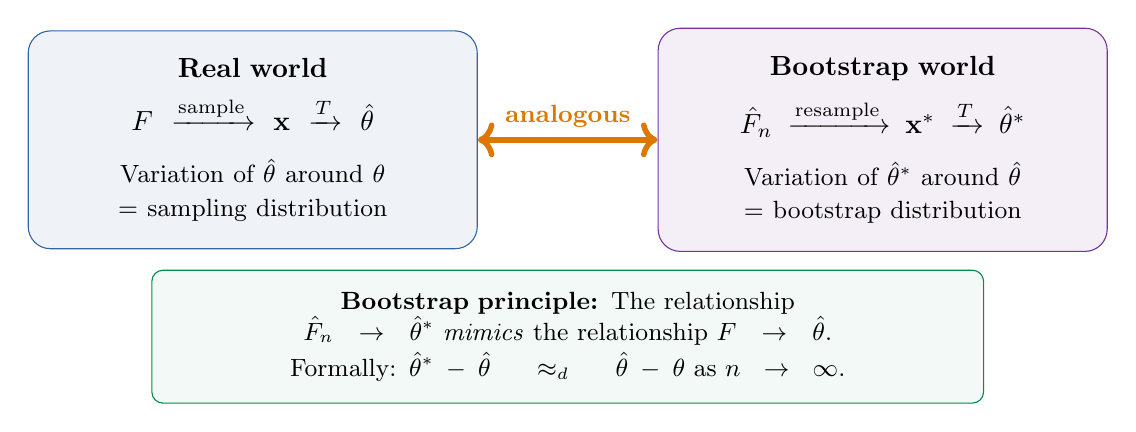
\begin{tikzpicture}
  % True world
  \node[draw=popblue, fill=popblue!8, rounded corners=8pt, text width=5cm, align=center, inner sep=10pt] (real) at (-4, 0) {
    \textbf{Real world}\\[6pt]
    $F \xrightarrow{\text{sample}} \mathbf{x} \xrightarrow{T} \hat\theta$\\[8pt]
    \small Variation of $\hat\theta$ around $\theta$\\
    $= $ sampling distribution
  };

  \node[draw=violet1, fill=violet1!8, rounded corners=8pt, text width=5cm, align=center, inner sep=10pt] (boot) at (4, 0) {
    \textbf{Bootstrap world}\\[6pt]
    $\hat{F}_n \xrightarrow{\text{resample}} \mathbf{x}^* \xrightarrow{T} \hat\theta^*$\\[8pt]
    \small Variation of $\hat\theta^*$ around $\hat\theta$\\
    $= $ bootstrap distribution
  };

  \draw[<->, very thick, orange1, line width=2pt] (real) -- (boot)
    node[midway, above, font=\small\bfseries] {analogous};

  % Bottom
  \node[draw=paramgreen, fill=paramgreen!5, rounded corners=4pt, text width=10cm, align=center, inner sep=8pt, font=\small] at (0, -2.5) {
    \textbf{Bootstrap principle:} The relationship $\hat{F}_n \to \hat\theta^*$ \textit{mimics} the relationship $F \to \hat\theta$.\\[2pt]
    Formally: $\hat\theta^* - \hat\theta \;\approx_d\; \hat\theta - \theta$ as $n \to \infty$.
  };
\end{tikzpicture}
\end{center}
\end{frame}

% ============================================================
\section{Bootstrap Confidence Intervals}

\begin{frame}
\begin{center}
  \vspace{2cm}
  {\Huge\bfseries\textcolor{popblue}{Bootstrap\\[0.3cm]Confidence Intervals}}

  \vspace{0.8cm}
  {\large Three methods, from simple to sophisticated}
\end{center}
\end{frame}

\begin{frame}
\frametitle{Method 1: The Normal Bootstrap CI}

\small
If the bootstrap distribution looks roughly Normal:

\vspace{0.2cm}
\begin{center}
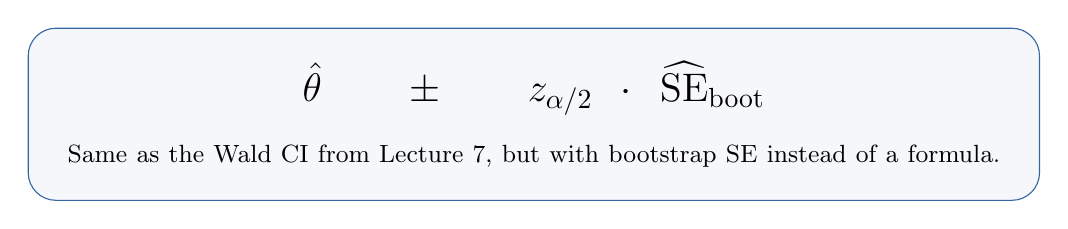
\begin{tikzpicture}
  \node[draw=popblue, fill=popblue!5, rounded corners=10pt, text width=12cm, align=center, inner sep=12pt] {
    {\Large $\hat\theta \;\pm\; z_{\alpha/2}\cdot \widehat{\text{SE}}_{\text{boot}}$}\\[10pt]
    \small Same as the Wald CI from Lecture~7, but with bootstrap SE instead of a formula.
  };
\end{tikzpicture}
\end{center}

\vspace{0.2cm}
\pause
\begin{center}
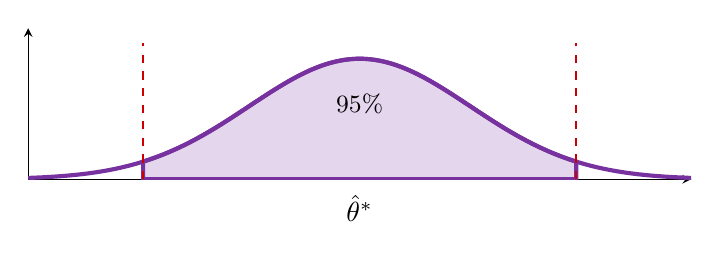
\begin{tikzpicture}
  \begin{axis}[
    width=10cm, height=3.5cm,
    xlabel={$\hat\theta^*$},
    ylabel={},
    axis lines=left,
    ytick=\empty,
    xtick=\empty,
    xmin=-3, xmax=3,
    ymin=0, ymax=0.5,
    every axis plot/.append style={line width=1.5pt, samples=100}
  ]
    \addplot[violet1, fill=violet1!20, domain=-1.96:1.96] {exp(-x^2/2)/sqrt(2*pi)} \closedcycle;
    \addplot[violet1, domain=-3:3] {exp(-x^2/2)/sqrt(2*pi)};

    \draw[thick, sampred, dashed] (axis cs:-1.96, 0) -- (axis cs:-1.96, 0.45);
    \draw[thick, sampred, dashed] (axis cs:1.96, 0) -- (axis cs:1.96, 0.45);
    \node[font=\small] at (axis cs:0, 0.25) {95\%};
  \end{axis}
\end{tikzpicture}
\end{center}

\vspace{-0.2cm}
\small\centering Simple, but assumes the bootstrap distribution is symmetric. Often it isn't!
\end{frame}

\begin{frame}
\frametitle{Method 2: The Percentile Bootstrap CI}

\begin{center}
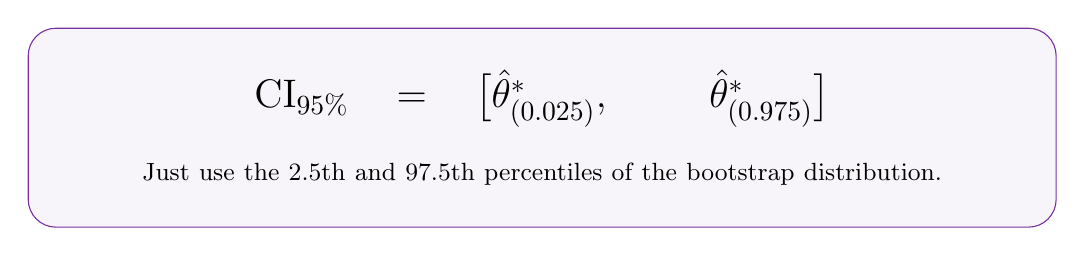
\begin{tikzpicture}
  \node[draw=violet1, fill=violet1!5, rounded corners=10pt, text width=12cm, align=center, inner sep=15pt] {
    {\Large
    $\text{CI}_{95\%} = \bigl[\hat\theta^*_{(0.025)},\;\; \hat\theta^*_{(0.975)}\bigr]$
    }\\[12pt]
    \small Just use the 2.5th and 97.5th percentiles of the bootstrap distribution.
  };
\end{tikzpicture}
\end{center}

\vspace{0.3cm}
\pause
\begin{center}
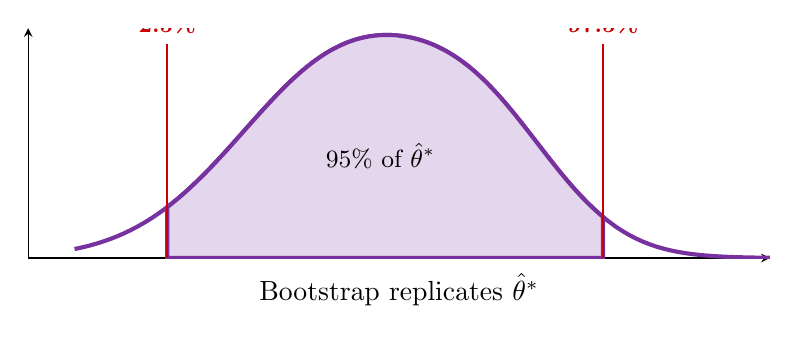
\begin{tikzpicture}
  \begin{axis}[
    width=11cm, height=4.5cm,
    xlabel={Bootstrap replicates $\hat\theta^*$},
    ylabel={},
    axis lines=left,
    ytick=\empty,
    xtick=\empty,
    xmin=-1, xmax=7,
    ymin=0, ymax=0.45,
    every axis plot/.append style={line width=1.5pt, samples=100}
  ]
    % Skewed distribution (log-normal-like)
    \addplot[violet1, domain=-0.5:7] {0.4*exp(-0.5*((x-2.5)/1.2)^2) + 0.15*exp(-0.5*((x-4)/0.8)^2)};
    \addplot[violet1, fill=violet1!20, domain=0.5:5.2] {0.4*exp(-0.5*((x-2.5)/1.2)^2) + 0.15*exp(-0.5*((x-4)/0.8)^2)} \closedcycle;

    \draw[thick, sampred] (axis cs:0.5, 0) -- (axis cs:0.5, 0.42);
    \node[font=\footnotesize\bfseries, sampred, above] at (axis cs:0.5, 0.42) {2.5\%};
    \draw[thick, sampred] (axis cs:5.2, 0) -- (axis cs:5.2, 0.42);
    \node[font=\footnotesize\bfseries, sampred, above] at (axis cs:5.2, 0.42) {97.5\%};

    \node[font=\small] at (axis cs:2.8, 0.2) {95\% of $\hat\theta^*$};
  \end{axis}
\end{tikzpicture}
\end{center}

\vspace{-0.1cm}
\small\centering
\textbf{Advantages:} respects asymmetry, no normality assumption, transformation-invariant.
\end{frame}

\begin{frame}
\frametitle{Method 3: BCa (Bias-Corrected and Accelerated)}

\small
The percentile method can have poor coverage when there is \textbf{bias} or \textbf{skewness}. The BCa interval adjusts the percentile cutoffs:

\vspace{0.2cm}
\begin{center}
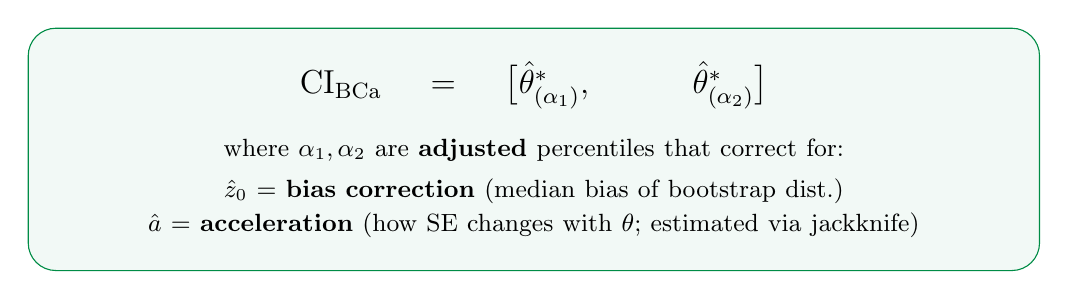
\begin{tikzpicture}
  \node[draw=paramgreen, fill=paramgreen!5, rounded corners=10pt, text width=12cm, align=center, inner sep=12pt] {
    {\large $\text{CI}_{\text{BCa}} = \bigl[\hat\theta^*_{(\alpha_1)},\;\; \hat\theta^*_{(\alpha_2)}\bigr]$}\\[10pt]
    \small where $\alpha_1, \alpha_2$ are \textbf{adjusted} percentiles that correct for:\\[4pt]
    $\hat{z}_0$ = \textbf{bias correction} (median bias of bootstrap dist.)\\
    $\hat{a}$ = \textbf{acceleration} (how SE changes with $\theta$; estimated via jackknife)
  };
\end{tikzpicture}
\end{center}

\vspace{0.3cm}
\pause
\begin{center}
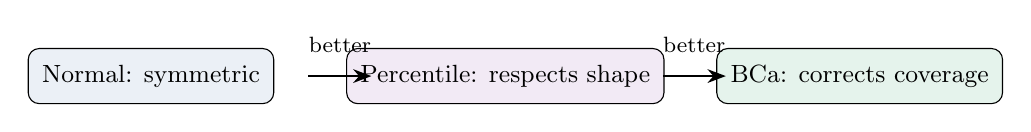
\begin{tikzpicture}[
  cbox/.style={draw, rounded corners=4pt, minimum height=0.7cm, align=center, font=\small, inner sep=5pt}
]
  \node[cbox, fill=popblue!10] at (-4.5, 0) {Normal: symmetric};
  \node[cbox, fill=violet1!10] at (0, 0) {Percentile: respects shape};
  \node[cbox, fill=paramgreen!10] at (4.5, 0) {BCa: corrects coverage};

  \draw[-{Stealth}, thick] (-2.5, 0) -- (-1.7, 0);
  \draw[-{Stealth}, thick] (2.0, 0) -- (2.8, 0);
  \node[font=\footnotesize] at (-2.1, 0.4) {better};
  \node[font=\footnotesize] at (2.4, 0.4) {better};
\end{tikzpicture}
\end{center}

\vspace{0.1cm}
\centering\small BCa is the \textbf{gold standard} for bootstrap CIs. Use it by default. Needs $B \geq 2{,}000$.
\end{frame}

\begin{frame}
\frametitle{Comparing Bootstrap CI Methods}

\begin{center}
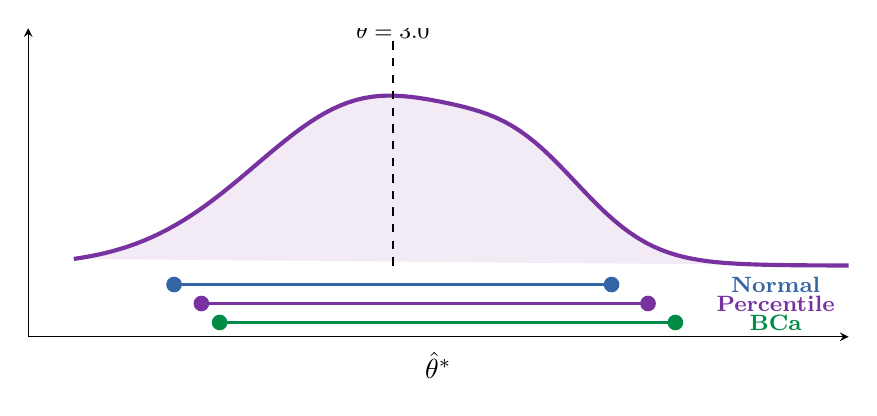
\begin{tikzpicture}
  \begin{axis}[
    width=12cm, height=5.5cm,
    xlabel={$\hat\theta^*$},
    ylabel={},
    axis lines=left,
    ytick=\empty,
    xtick=\empty,
    xmin=-1, xmax=8,
    ymin=-0.15, ymax=0.5,
    every axis plot/.append style={line width=1.5pt, samples=100}
  ]
    % Skewed bootstrap distribution
    \addplot[violet1, fill=violet1!10, domain=-0.5:8] {
      0.35*exp(-0.5*((x-2.8)/1.3)^2) + 0.12*exp(-0.5*((x-4.5)/0.7)^2)
    };

    % Original estimate
    \draw[thick, black, dashed] (axis cs:3, 0) -- (axis cs:3, 0.48);
    \node[font=\footnotesize\bfseries] at (axis cs:3, 0.5) {$\hat\theta = 3.0$};

    % Normal CI (symmetric, misses skew)
    \draw[very thick, popblue] (axis cs:0.6, -0.04) -- (axis cs:5.4, -0.04);
    \node[circle, fill=popblue, inner sep=2pt] at (axis cs:0.6, -0.04) {};
    \node[circle, fill=popblue, inner sep=2pt] at (axis cs:5.4, -0.04) {};
    \node[font=\footnotesize\bfseries, popblue] at (axis cs:7.2, -0.04) {Normal};

    % Percentile CI (shifted right)
    \draw[very thick, violet1] (axis cs:0.9, -0.08) -- (axis cs:5.8, -0.08);
    \node[circle, fill=violet1, inner sep=2pt] at (axis cs:0.9, -0.08) {};
    \node[circle, fill=violet1, inner sep=2pt] at (axis cs:5.8, -0.08) {};
    \node[font=\footnotesize\bfseries, violet1] at (axis cs:7.2, -0.08) {Percentile};

    % BCa CI (best coverage)
    \draw[very thick, paramgreen] (axis cs:1.1, -0.12) -- (axis cs:6.1, -0.12);
    \node[circle, fill=paramgreen, inner sep=2pt] at (axis cs:1.1, -0.12) {};
    \node[circle, fill=paramgreen, inner sep=2pt] at (axis cs:6.1, -0.12) {};
    \node[font=\footnotesize\bfseries, paramgreen] at (axis cs:7.2, -0.12) {BCa};
  \end{axis}
\end{tikzpicture}
\end{center}

\small
When the bootstrap distribution is \textbf{skewed}, the three methods give different intervals.\\
The Normal CI is symmetric around $\hat\theta$ and can miss the tail. BCa adapts to the shape.
\end{frame}

% ============================================================
\section{Parametric vs Nonparametric Bootstrap}

\begin{frame}
\begin{center}
  \vspace{2cm}
  {\Huge\bfseries\textcolor{popblue}{Parametric vs\\[0.3cm]Nonparametric Bootstrap}}

  \vspace{0.8cm}
  {\large Two flavors of resampling}
\end{center}
\end{frame}

\begin{frame}
\frametitle{Two Flavors of Bootstrap}

\begin{center}
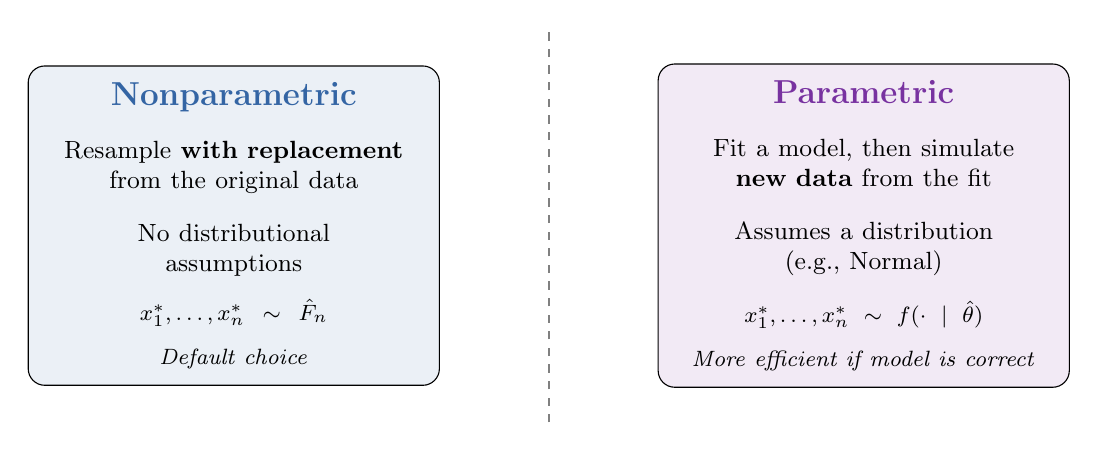
\begin{tikzpicture}[
  fbox/.style={draw, rounded corners=6pt, minimum width=5cm, minimum height=4cm, align=center, text width=4.8cm, inner sep=6pt}
]
  \node[fbox, fill=popblue!10] at (-4, 0) {
    \textbf{\large\textcolor{popblue}{Nonparametric}}\\[8pt]
    \small Resample \textbf{with replacement}\\
    from the original data\\[8pt]
    No distributional\\assumptions\\[8pt]
    \footnotesize $x_1^*, \ldots, x_n^* \sim \hat{F}_n$\\[4pt]
    \textit{Default choice}
  };

  \node[fbox, fill=violet1!10] at (4, 0) {
    \textbf{\large\textcolor{violet1}{Parametric}}\\[8pt]
    \small Fit a model, then simulate\\
    \textbf{new data} from the fit\\[8pt]
    Assumes a distribution\\(e.g., Normal)\\[8pt]
    \footnotesize $x_1^*, \ldots, x_n^* \sim f(\cdot \mid \hat\theta)$\\[4pt]
    \textit{More efficient if model is correct}
  };

  \draw[thick, gray, dashed] (0, -2.5) -- (0, 2.5);
\end{tikzpicture}
\end{center}

\vspace{0.2cm}
\pause
\centering\small
\textbf{Rule of thumb:} Use nonparametric unless you have strong reasons to trust the model.
\end{frame}

\begin{frame}
\frametitle{Example: Bootstrap SE of the Correlation}

\small
Data: $(x_i, y_i)$ for $i = 1, \ldots, n$. \; Statistic: $\hat{r} = \text{Cor}(x, y) = 0.68$.

\vspace{0.1cm}
There's a formula for SE (Fisher's $z$-transform), but the bootstrap gives it for free:

\vspace{0.2cm}
\begin{center}
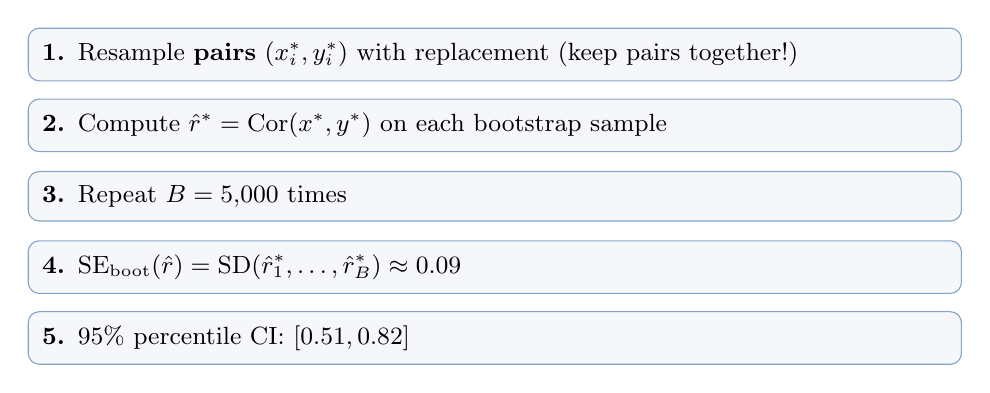
\begin{tikzpicture}[
  stp/.style={draw=popblue!60, fill=popblue!5, rounded corners=4pt, text width=11.5cm, minimum height=0.55cm, align=left, inner sep=5pt, font=\small}
]
  \node[stp] at (0, 1.6) {\textbf{1.} Resample \textbf{pairs} $(x_i^*, y_i^*)$ with replacement (keep pairs together!)};
  \node[stp] at (0, 0.7) {\textbf{2.} Compute $\hat{r}^* = \text{Cor}(x^*, y^*)$ on each bootstrap sample};
  \node[stp] at (0, -0.2) {\textbf{3.} Repeat $B = 5{,}000$ times};
  \node[stp] at (0, -1.1) {\textbf{4.} $\text{SE}_{\text{boot}}(\hat{r}) = \text{SD}(\hat{r}_1^*, \ldots, \hat{r}_B^*) \approx 0.09$};
  \node[stp] at (0, -2.0) {\textbf{5.} 95\% percentile CI: $[0.51, 0.82]$};
\end{tikzpicture}
\end{center}

\vspace{0.2cm}
\pause
\begin{center}
\fcolorbox{warnred}{warnred!5}{\parbox{10cm}{\centering\small
  \textbf{Important:} Resample the \textit{pairs}, not $x$ and $y$ separately!\\[2pt]
  Resampling them independently would destroy the correlation structure.
}}
\end{center}
\end{frame}

% ============================================================
\section{When Bootstrap Fails}

\begin{frame}
\begin{center}
  \vspace{2cm}
  {\Huge\bfseries\textcolor{popblue}{When Bootstrap Fails}}

  \vspace{0.8cm}
  {\large It's not magic --- it has limits}
\end{center}
\end{frame}

\begin{frame}
\frametitle{When the Bootstrap Fails}

\begin{center}
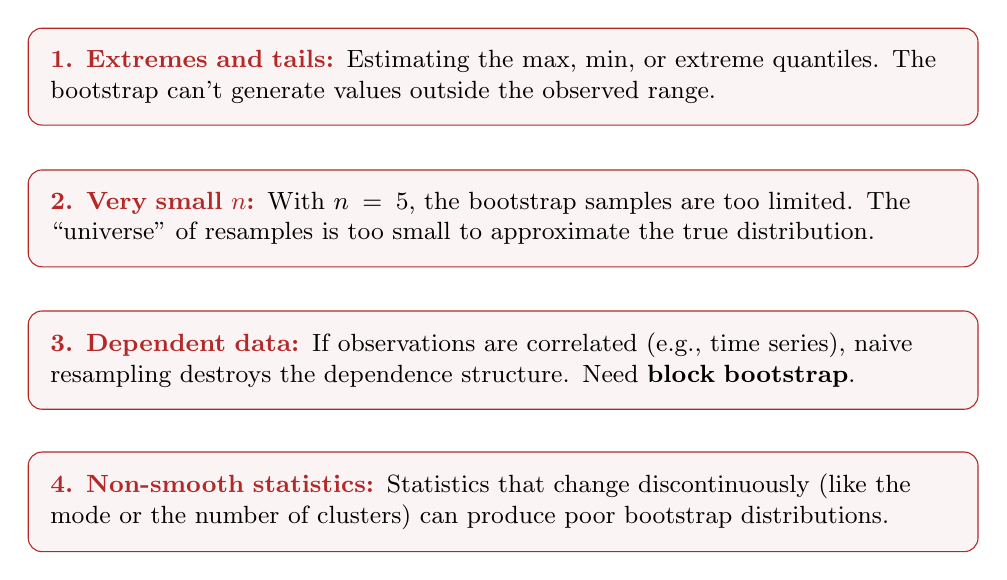
\begin{tikzpicture}[
  fbox/.style={draw=warnred, fill=warnred!5, rounded corners=5pt, text width=11.5cm, minimum height=1.1cm, align=left, inner sep=8pt, font=\small}
]
  \node[fbox] at (0, 3) {
    \textbf{\textcolor{warnred}{1. Extremes and tails:}} Estimating the max, min, or extreme quantiles. The bootstrap can't generate values outside the observed range.
  };
  \pause
  \node[fbox] at (0, 1.2) {
    \textbf{\textcolor{warnred}{2. Very small $n$:}} With $n = 5$, the bootstrap samples are too limited. The ``universe'' of resamples is too small to approximate the true distribution.
  };
  \pause
  \node[fbox] at (0, -0.6) {
    \textbf{\textcolor{warnred}{3. Dependent data:}} If observations are correlated (e.g., time series), naive resampling destroys the dependence structure. Need \textbf{block bootstrap}.
  };
  \pause
  \node[fbox] at (0, -2.4) {
    \textbf{\textcolor{warnred}{4. Non-smooth statistics:}} Statistics that change discontinuously (like the mode or the number of clusters) can produce poor bootstrap distributions.
  };
\end{tikzpicture}
\end{center}
\end{frame}

\begin{frame}
\frametitle{Bootstrap Fails for Extremes: Why?}

\small
\textbf{Example:} $X_1, \ldots, X_n \sim \text{Uniform}(0, \theta)$. Estimate $\hat\theta = X_{(n)} = \max(X_i)$.

\vspace{0.2cm}
\begin{center}
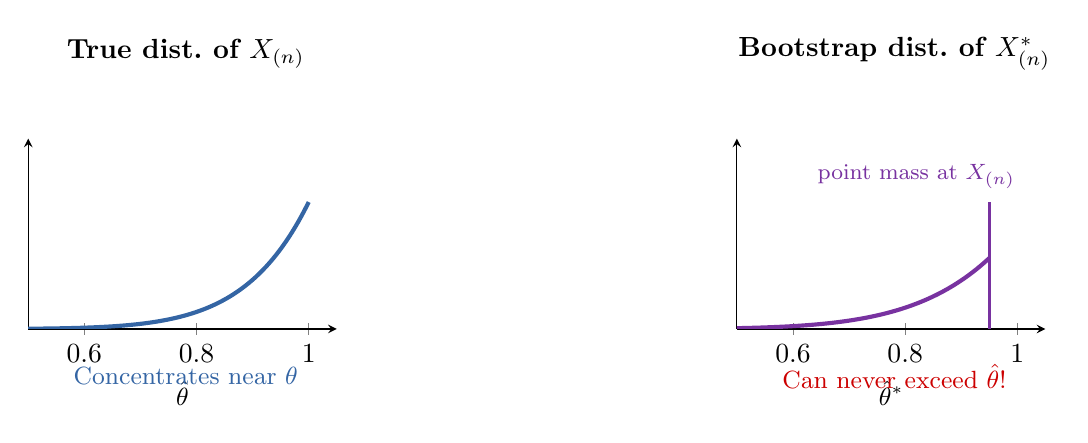
\begin{tikzpicture}
  % Left: true sampling distribution of max
  \begin{scope}[xshift=-4.5cm]
    \node[font=\bfseries] at (2, 3.5) {True dist.\ of $X_{(n)}$};
    \begin{axis}[
      width=5.5cm, height=4cm,
      xmin=0.5, xmax=1.05, ymin=0, ymax=15,
      axis lines=left,
      xtick={0.6, 0.8, 1.0}, ytick=\empty,
      xlabel={\small $\hat\theta$},
      every axis plot/.append style={line width=1.5pt, samples=80},
      at={(0,0)}
    ]
      % True: n*x^(n-1) concentrated near theta=1, n=10
      \addplot[popblue, domain=0.5:1] {10*x^9};
    \end{axis}
    \node[font=\small, popblue] at (2, -0.6) {Concentrates near $\theta$};
  \end{scope}

  % Right: bootstrap distribution of max
  \begin{scope}[xshift=4.5cm]
    \node[font=\bfseries] at (2, 3.5) {Bootstrap dist.\ of $X^*_{(n)}$};
    \begin{axis}[
      width=5.5cm, height=4cm,
      xmin=0.5, xmax=1.05, ymin=0, ymax=15,
      axis lines=left,
      xtick={0.6, 0.8, 1.0}, ytick=\empty,
      xlabel={\small $\hat\theta^*$},
      every axis plot/.append style={line width=1.5pt, samples=80},
      at={(0,0)}
    ]
      % Bootstrap: can never exceed X_(n), has a point mass at X_(n)
      \addplot[violet1, domain=0.5:0.95] {8*x^7};
      \draw[very thick, violet1] (axis cs:0.95, 0) -- (axis cs:0.95, 10);
      \node[font=\footnotesize, violet1] at (axis cs:0.82, 12) {point mass at $X_{(n)}$};
    \end{axis}
    \node[font=\small, sampred] at (2, -0.6) {Can never exceed $\hat\theta$!};
  \end{scope}
\end{tikzpicture}
\end{center}

\vspace{0.1cm}
\centering\small
The bootstrap \textbf{underestimates} the variability of $X_{(n)}$ because it can't generate values beyond the observed maximum. Same issue from Lecture~5 (MLE for Uniform).
\end{frame}

% ============================================================
\section{Permutation Tests}

\begin{frame}
\begin{center}
  \vspace{2cm}
  {\Huge\bfseries\textcolor{popblue}{Permutation Tests}}

  \vspace{0.8cm}
  {\large Resampling for hypothesis testing}
\end{center}
\end{frame}

\begin{frame}
\frametitle{The Permutation Test Idea}

\small
\textbf{Question:} Is there a real difference between Group A and Group B?

\vspace{0.1cm}
\begin{center}
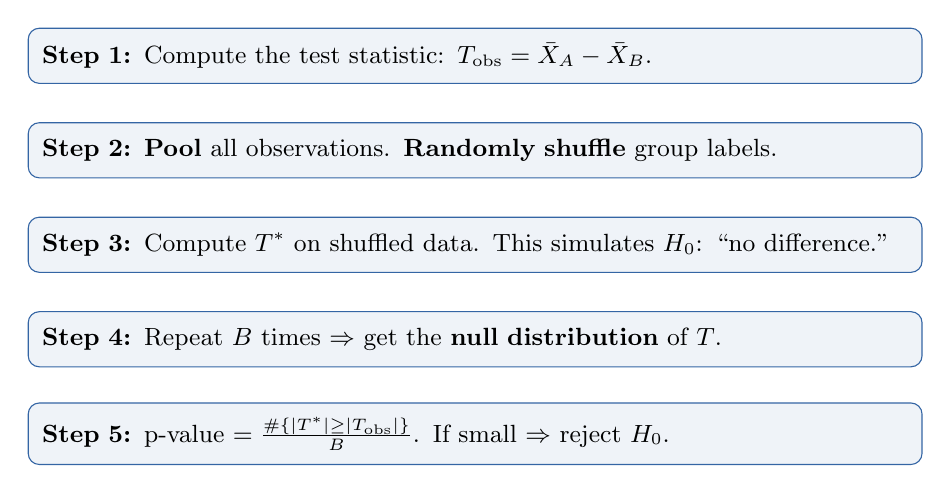
\begin{tikzpicture}[
  stp/.style={draw=popblue, fill=popblue!8, rounded corners=4pt, text width=11cm, minimum height=0.7cm, align=left, inner sep=5pt, font=\small}
]
  \node[stp] at (0, 2.5) {\textbf{Step 1:} Compute the test statistic: $T_{\text{obs}} = \bar{X}_A - \bar{X}_B$.};
  \pause
  \node[stp] at (0, 1.3) {\textbf{Step 2:} \textbf{Pool} all observations. \textbf{Randomly shuffle} group labels.};
  \pause
  \node[stp] at (0, 0.1) {\textbf{Step 3:} Compute $T^*$ on shuffled data. This simulates $H_0$: ``no difference.''};
  \pause
  \node[stp] at (0, -1.1) {\textbf{Step 4:} Repeat $B$ times $\Rightarrow$ get the \textbf{null distribution} of $T$.};
  \pause
  \node[stp] at (0, -2.3) {\textbf{Step 5:} p-value $= \frac{\#\{|T^*| \geq |T_{\text{obs}}|\}}{B}$. If small $\Rightarrow$ reject $H_0$.};
\end{tikzpicture}
\end{center}
\end{frame}

\begin{frame}
\frametitle{Permutation Test: Visual Example}

\small
\textbf{Drug trial:} Treatment ($n_A = 8$, mean = 5.2) vs Control ($n_B = 8$, mean = 3.1). \;$T_{\text{obs}} = 2.1$.

\vspace{0.2cm}
\begin{center}
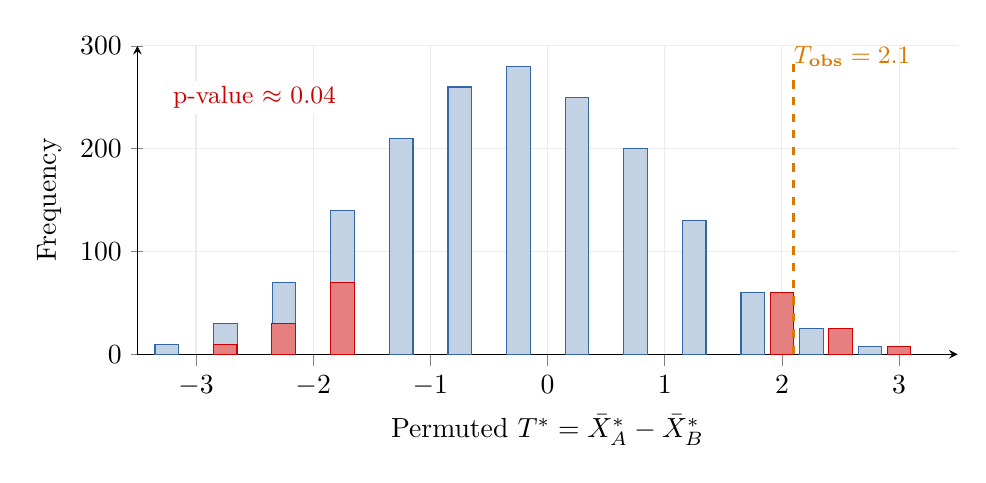
\begin{tikzpicture}
  \begin{axis}[
    width=12cm, height=5.5cm,
    xlabel={Permuted $T^* = \bar{X}_A^* - \bar{X}_B^*$},
    ylabel={Frequency},
    xmin=-3.5, xmax=3.5,
    ymin=0, ymax=300,
    axis lines=left,
    grid=major, grid style={gray!15},
    bar width=0.3cm,
    ybar,
  ]
    % Null distribution (approximately normal, centered at 0)
    \addplot[fill=popblue!30, draw=popblue] coordinates {
      (-3.0, 10) (-2.5, 30) (-2.0, 70) (-1.5, 140) (-1.0, 210)
      (-0.5, 260) (0.0, 280) (0.5, 250) (1.0, 200) (1.5, 130)
      (2.0, 60) (2.5, 25) (3.0, 8)
    };

    % Rejection region
    \addplot[fill=sampred!50, draw=sampred] coordinates {
      (2.0, 60) (2.5, 25) (3.0, 8)
    };
    \addplot[fill=sampred!50, draw=sampred] coordinates {
      (-3.0, 10) (-2.5, 30) (-2.0, 70)
    };

    % Observed value
    \draw[very thick, orange1, dashed] (axis cs:2.1, 0) -- (axis cs:2.1, 290);
    \node[font=\small\bfseries, orange1] at (axis cs:2.6, 290) {$T_{\text{obs}} = 2.1$};

    % p-value annotation
    \node[font=\small, sampred, fill=white, inner sep=2pt] at (axis cs:-2.5, 250) {p-value $\approx$ 0.04};
  \end{axis}
\end{tikzpicture}
\end{center}

\vspace{-0.1cm}
\centering\small
Only $\sim$4\% of shuffled datasets produce a difference $\geq 2.1$. The drug effect is likely real.
\end{frame}

\begin{frame}
\frametitle{Bootstrap vs Permutation: What's the Difference?}

\begin{center}
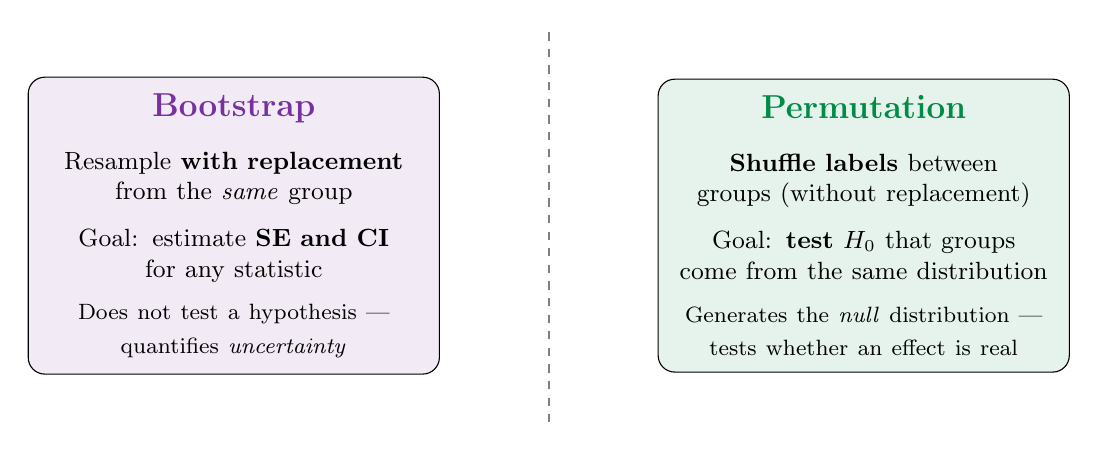
\begin{tikzpicture}[
  cbox/.style={draw, rounded corners=6pt, minimum width=5cm, minimum height=3.5cm, align=center, text width=4.8cm, inner sep=6pt}
]
  \node[cbox, fill=violet1!10] at (-4, 0) {
    \textbf{\large\textcolor{violet1}{Bootstrap}}\\[8pt]
    \small Resample \textbf{with replacement}\\
    from the \textit{same} group\\[6pt]
    Goal: estimate \textbf{SE and CI}\\
    for any statistic\\[6pt]
    \footnotesize Does not test a hypothesis ---\\
    quantifies \textit{uncertainty}
  };

  \node[cbox, fill=paramgreen!10] at (4, 0) {
    \textbf{\large\textcolor{paramgreen}{Permutation}}\\[8pt]
    \small \textbf{Shuffle labels} between\\
    groups (without replacement)\\[6pt]
    Goal: \textbf{test $H_0$} that groups\\
    come from the same distribution\\[6pt]
    \footnotesize Generates the \textit{null} distribution ---\\
    tests whether an effect is real
  };

  \draw[thick, gray, dashed] (0, -2.5) -- (0, 2.5);
\end{tikzpicture}
\end{center}

\vspace{0.2cm}
\centering\small
Bootstrap answers: ``How precise is my estimate?'' \; Permutation answers: ``Is there an effect?''
\end{frame}

% ============================================================
\section{Practical Considerations}

\begin{frame}
\begin{center}
  \vspace{2cm}
  {\Huge\bfseries\textcolor{popblue}{Practical\\[0.3cm]Considerations}}

  \vspace{0.8cm}
  {\large Making it work in practice}
\end{center}
\end{frame}

\begin{frame}
\frametitle{How Many Bootstrap Replicates?}

\begin{center}
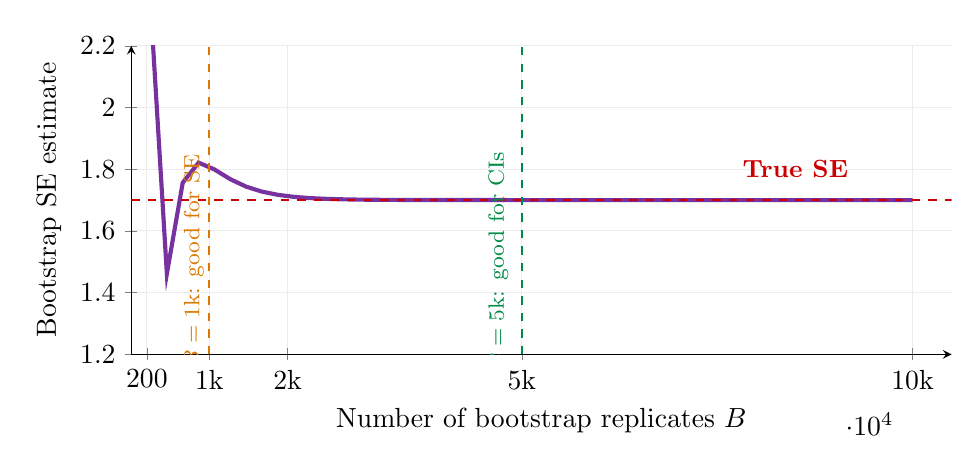
\begin{tikzpicture}
  \begin{axis}[
    width=12cm, height=5.5cm,
    xlabel={Number of bootstrap replicates $B$},
    ylabel={Bootstrap SE estimate},
    xmin=0, xmax=10500,
    ymin=1.2, ymax=2.2,
    axis lines=left,
    grid=major, grid style={gray!15},
    xtick={200, 1000, 2000, 5000, 10000},
    xticklabels={200, $1\text{k}$, $2\text{k}$, $5\text{k}$, $10\text{k}$},
    every axis plot/.append style={line width=1.5pt, samples=50}
  ]
    % SE estimate stabilizes
    \addplot[violet1, domain=50:10000] {1.7 + 0.8*sin(deg(20/x*100))*exp(-x/500) + 0.3*exp(-x/300)};

    % True value
    \draw[thick, sampred, dashed] (axis cs:0, 1.7) -- (axis cs:10500, 1.7);
    \node[font=\small\bfseries, sampred] at (axis cs:8500, 1.8) {True SE};

    % Annotations
    \draw[thick, orange1, dashed] (axis cs:1000, 1.2) -- (axis cs:1000, 2.2);
    \node[font=\footnotesize, orange1, rotate=90] at (axis cs:800, 1.5) {$B = 1\text{k}$: good for SE};

    \draw[thick, paramgreen, dashed] (axis cs:5000, 1.2) -- (axis cs:5000, 2.2);
    \node[font=\footnotesize, paramgreen, rotate=90] at (axis cs:4700, 1.5) {$B = 5\text{k}$: good for CIs};
  \end{axis}
\end{tikzpicture}
\end{center}

\small
\textbf{Rules of thumb:} $B \geq 200$ for SE, $B \geq 1{,}000$ for percentile CI, $B \geq 5{,}000$ for BCa CI.
\end{frame}

\begin{frame}
\frametitle{Bootstrap in Python: It's Simple}

\begin{center}
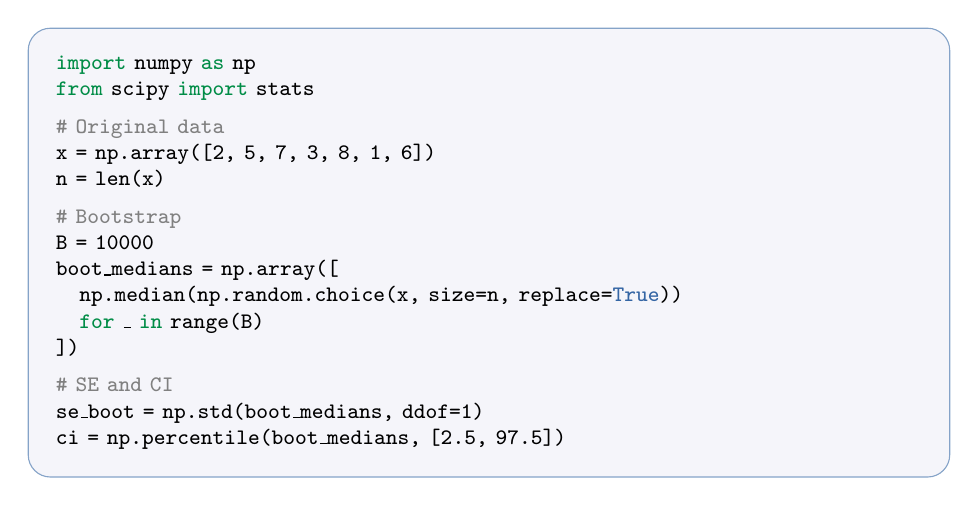
\begin{tikzpicture}
  \node[draw=popblue!60, fill=lightbg, rounded corners=8pt, text width=11cm, align=left, inner sep=10pt, font=\ttfamily\footnotesize] {
    \textcolor{paramgreen}{import} numpy \textcolor{paramgreen}{as} np\\
    \textcolor{paramgreen}{from} scipy \textcolor{paramgreen}{import} stats\\[4pt]
    \textcolor{gray}{\# Original data}\\
    x = np.array([2, 5, 7, 3, 8, 1, 6])\\
    n = len(x)\\[4pt]
    \textcolor{gray}{\# Bootstrap}\\
    B = 10000\\
    boot\_medians = np.array([\\
    \quad np.median(np.random.choice(x, size=n, replace=\textcolor{popblue}{True}))\\
    \quad \textcolor{paramgreen}{for} \_ \textcolor{paramgreen}{in} range(B)\\
    ])\\[4pt]
    \textcolor{gray}{\# SE and CI}\\
    se\_boot = np.std(boot\_medians, ddof=1)\\
    ci = np.percentile(boot\_medians, [2.5, 97.5])
  };
\end{tikzpicture}
\end{center}

\vspace{0.1cm}
\centering\small
For BCa: use \texttt{scipy.stats.bootstrap()} (since SciPy 1.7) or \texttt{arch.bootstrap}.
\end{frame}

% ============================================================
\section{Summary}

\begin{frame}
\frametitle{Summary: The Bootstrap Toolbox}
\begin{center}
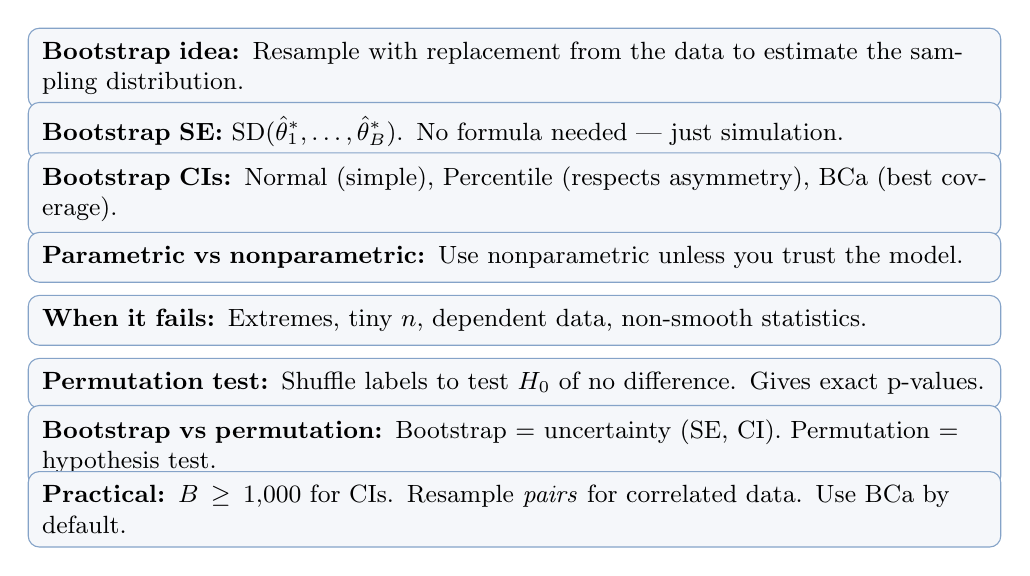
\begin{tikzpicture}[
  sbox/.style={draw=popblue!60, fill=popblue!5, rounded corners=4pt, text width=12cm, minimum height=0.5cm, align=left, inner sep=5pt, font=\small}
]
  \node[sbox] at (0, 3.2) {\textbf{Bootstrap idea:} Resample with replacement from the data to estimate the sampling distribution.};
  \node[sbox] at (0, 2.4) {\textbf{Bootstrap SE:} $\text{SD}(\hat\theta_1^*, \ldots, \hat\theta_B^*)$. No formula needed --- just simulation.};
  \node[sbox] at (0, 1.6) {\textbf{Bootstrap CIs:} Normal (simple), Percentile (respects asymmetry), BCa (best coverage).};
  \node[sbox] at (0, 0.8) {\textbf{Parametric vs nonparametric:} Use nonparametric unless you trust the model.};
  \node[sbox] at (0, 0.0) {\textbf{When it fails:} Extremes, tiny $n$, dependent data, non-smooth statistics.};
  \node[sbox] at (0, -0.8) {\textbf{Permutation test:} Shuffle labels to test $H_0$ of no difference. Gives exact p-values.};
  \node[sbox] at (0, -1.6) {\textbf{Bootstrap vs permutation:} Bootstrap = uncertainty (SE, CI). Permutation = hypothesis test.};
  \node[sbox] at (0, -2.4) {\textbf{Practical:} $B \geq 1{,}000$ for CIs. Resample \textit{pairs} for correlated data. Use BCa by default.};
\end{tikzpicture}
\end{center}
\end{frame}

% ============================================================
\section{Practical}

\begin{frame}
\frametitle{Practical: Bootstrap in Action}
\begin{center}
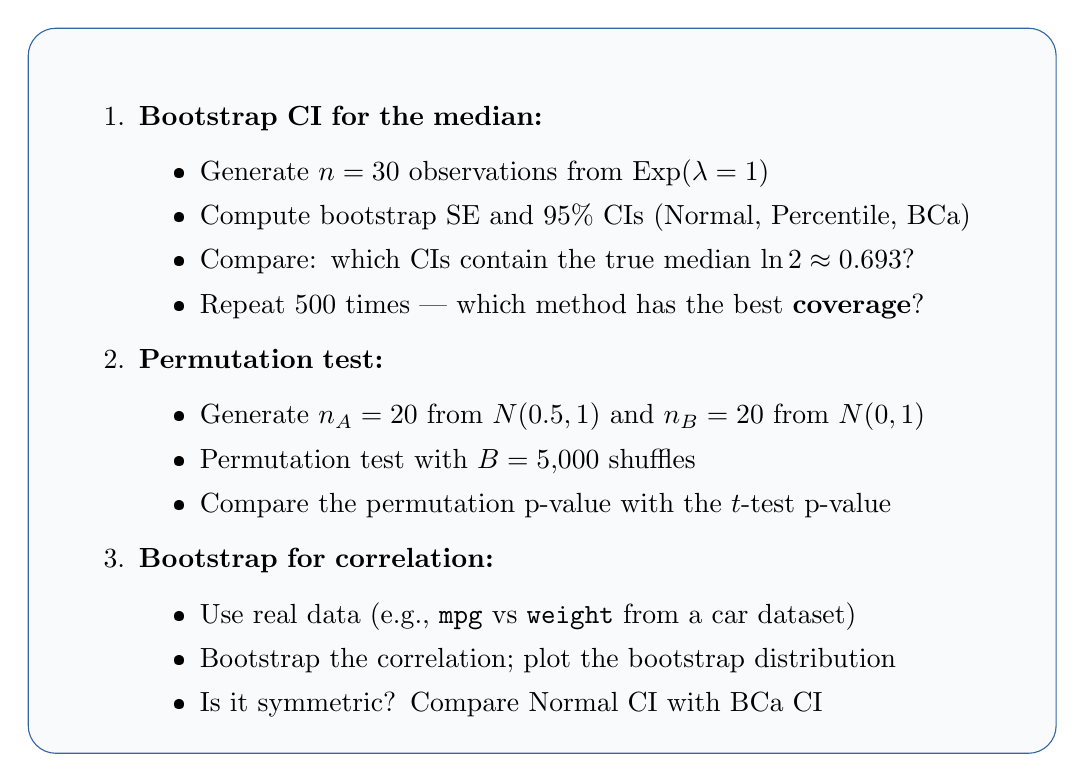
\begin{tikzpicture}
  \node[draw=popblue, fill=popblue!3, rounded corners=10pt, text width=12cm, align=left, inner sep=15pt] {
    \begin{enumerate}
      \item \textbf{Bootstrap CI for the median:}
        \begin{itemize}
          \item Generate $n = 30$ observations from $\text{Exp}(\lambda = 1)$
          \item Compute bootstrap SE and 95\% CIs (Normal, Percentile, BCa)
          \item Compare: which CIs contain the true median $\ln 2 \approx 0.693$?
          \item Repeat 500 times --- which method has the best \textbf{coverage}?
        \end{itemize}
      \item \textbf{Permutation test:}
        \begin{itemize}
          \item Generate $n_A = 20$ from $N(0.5, 1)$ and $n_B = 20$ from $N(0, 1)$
          \item Permutation test with $B = 5{,}000$ shuffles
          \item Compare the permutation p-value with the $t$-test p-value
        \end{itemize}
      \item \textbf{Bootstrap for correlation:}
        \begin{itemize}
          \item Use real data (e.g., \texttt{mpg} vs \texttt{weight} from a car dataset)
          \item Bootstrap the correlation; plot the bootstrap distribution
          \item Is it symmetric? Compare Normal CI with BCa CI
        \end{itemize}
    \end{enumerate}
  };
\end{tikzpicture}
\end{center}
\end{frame}

\begin{frame}
\frametitle{Homework}
\begin{enumerate}
  \item The heights (cm) of 12 students are: 165, 170, 168, 172, 175, 180, 163, 178, 169, 171, 167, 174.\\
    (a) Compute the bootstrap SE of the median using $B = 5{,}000$.\\
    (b) Construct 95\% Normal and Percentile bootstrap CIs.\\
    (c) Is the bootstrap distribution symmetric? Why or why not?

  \vspace{0.1cm}
  \item Show that the bootstrap estimate of SE$(\bar{X})$ converges to $S/\sqrt{n}$ as $B \to \infty$.\\
    \textit{Hint:} What is the variance of sampling with replacement from a finite set?

  \vspace{0.1cm}
  \item A/B test: Group A (50 users, mean revenue \$12.50, SD \$8.00) vs Group B (50 users, mean \$14.20, SD \$9.50).\\
    (a) Perform a permutation test for $H_0$: no difference in means.\\
    (b) Compute a bootstrap CI for the \textit{difference} in means.\\
    (c) Do the two approaches agree?

  \vspace{0.1cm}
  \item Why does the bootstrap fail for $\hat\theta = X_{(n)}$ when $X_i \sim \text{Uniform}(0, \theta)$?\\
    Show that the bootstrap distribution of $X^*_{(n)}$ has a point mass at $X_{(n)}$ of size $(1 - 1/n)^n \to 1/e$.
\end{enumerate}
\end{frame}

\begin{frame}
\frametitle{Recommended Visualizations \& Resources}

\small
\begin{center}
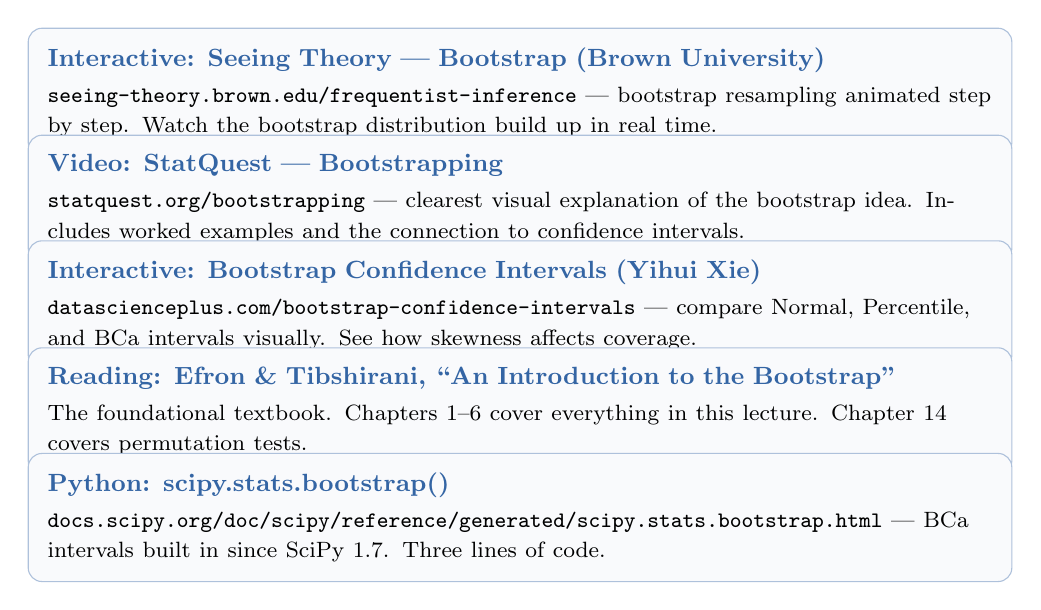
\begin{tikzpicture}[
  rbox/.style={draw=popblue!40, fill=popblue!3, rounded corners=5pt, text width=12cm, align=left, inner sep=7pt, font=\small}
]
  \node[rbox] at (0, 2.7) {
    \textbf{\textcolor{popblue}{Interactive: Seeing Theory --- Bootstrap (Brown University)}}\\[2pt]
    \footnotesize\texttt{seeing-theory.brown.edu/frequentist-inference} --- bootstrap resampling animated step by step. Watch the bootstrap distribution build up in real time.
  };
  \node[rbox] at (0, 1.35) {
    \textbf{\textcolor{popblue}{Video: StatQuest --- Bootstrapping}}\\[2pt]
    \footnotesize\texttt{statquest.org/bootstrapping} --- clearest visual explanation of the bootstrap idea. Includes worked examples and the connection to confidence intervals.
  };
  \node[rbox] at (0, 0.0) {
    \textbf{\textcolor{popblue}{Interactive: Bootstrap Confidence Intervals (Yihui Xie)}}\\[2pt]
    \footnotesize\texttt{datascienceplus.com/bootstrap-confidence-intervals} --- compare Normal, Percentile, and BCa intervals visually. See how skewness affects coverage.
  };
  \node[rbox] at (0, -1.35) {
    \textbf{\textcolor{popblue}{Reading: Efron \& Tibshirani, ``An Introduction to the Bootstrap''}}\\[2pt]
    \footnotesize The foundational textbook. Chapters 1--6 cover everything in this lecture. Chapter 14 covers permutation tests.
  };
  \node[rbox] at (0, -2.7) {
    \textbf{\textcolor{popblue}{Python: scipy.stats.bootstrap()}}\\[2pt]
    \footnotesize\texttt{docs.scipy.org/doc/scipy/reference/generated/scipy.stats.bootstrap.html} --- BCa intervals built in since SciPy 1.7. Three lines of code.
  };
\end{tikzpicture}
\end{center}
\end{frame}

\begin{frame}
\begin{center}
  {\Huge\bfseries\textcolor{popblue}{Questions?}}

  \vspace{1cm}

  {\large Next: Lecture~9 --- Hypothesis testing, p-values, and power}
\end{center}
\end{frame}

\end{document}
